\documentclass{article}
\usepackage{../proto-docs}
\usepackage{fullpage}
\usepackage{graphicx}
\usepackage{../svn-multi}

\title{MIT Proto Compiler Developers Guide}
\author{By the authors of MIT Proto}
\date{\releasetag}

\newcommand\todo[1]{\immediate\write16{TODO: #1}}

\newcommand\fixme{{\bf NEEDS DEVELOPER ATTENTION}}

\newcommand\file[1]{{\tt #1}}

% proto code
\newcommand\code[1]{\begin{quote}\var{#1}\end{quote}}
\newcommand\function[2]
{\begin{quote}{\tt #1}: #2 \end{quote}}
\newcommand\type[1]{$#1$}
\newcommand\var[1]{{\tt #1}}

\begin{document}

\maketitle

This is a guide to Proto compilation, as implemented in MIT Proto. It outlines
the various components of the compiler, how they fit together, and how to
develop for them safely.  For more general developer documentation, see the {\bf
MIT Proto Developers Guide}.  For user documentation, begin with the {\bf Proto
Quick Start}. For installation instructions, see the {\bf README}.

WARNING: This file is still highly incomplete.

\tableofcontents

\credits{}

\section{Neocompiler vs. Paleocompiler}

MIT Proto has had two compilers.  The first implementation, the
``paleocompiler,'' grew organically along with the development of the Proto
language, and is tightly wrapped around compilation to the ProtoKernel VM.
Because there was no well-defined semantics for Proto for most of its
development, it never actually represents a Proto computation explicitly,
translating a number of operations directly into ProtoKernel constructs.  This
resulted in some fundamental hard-to-repair bugs, a major limitation in the
ability to upgrade the compiler to match development in the language, and the
inability to compile to any other platform besides the ProtoKernel VM.

In late 2009, a complete rebuild of the compiler was begun, motivated by the
desire to compile Proto programs to genetic regulatory networks for inclusion in
living cells.  This new compiler is based around a precise representation of
Proto's dataflow computation semantics. This variant, the ``neocompiler,'' is
not yet complete as of this writing.  As such, the neocompiler and paleocompiler
are both maintained and built into the MIT Proto distribution.  When the
neocompiler fully implements all capabilities of the paleocompiler, the
paleocompiler will be deprecated, then eventually removed from the distribution.

The neocompiler's current major limitations are:
\begin{itemize}
  \item Function calls are not emitted correctly.
  \item Space-time operators are not compiled from global to local.
  \item Functions cannot be recursive.
  \item Compiler/simulator plugins cannot add their own opcodes.
\end{itemize}
However, the neocompiler is where the future of Proto is inevitably bound, and
is the focus of almost all present development work on the Proto compiler.  As
such, this guide will focus almost entirely on the neocompiler, which we shall
refer to simply as the compiler.

One final note: when files are referred to, they are assumed to be in the
\file{src/compiler/} directory of the MIT Proto distribution unless otherwise
specified.

\begin{figure}
\centering
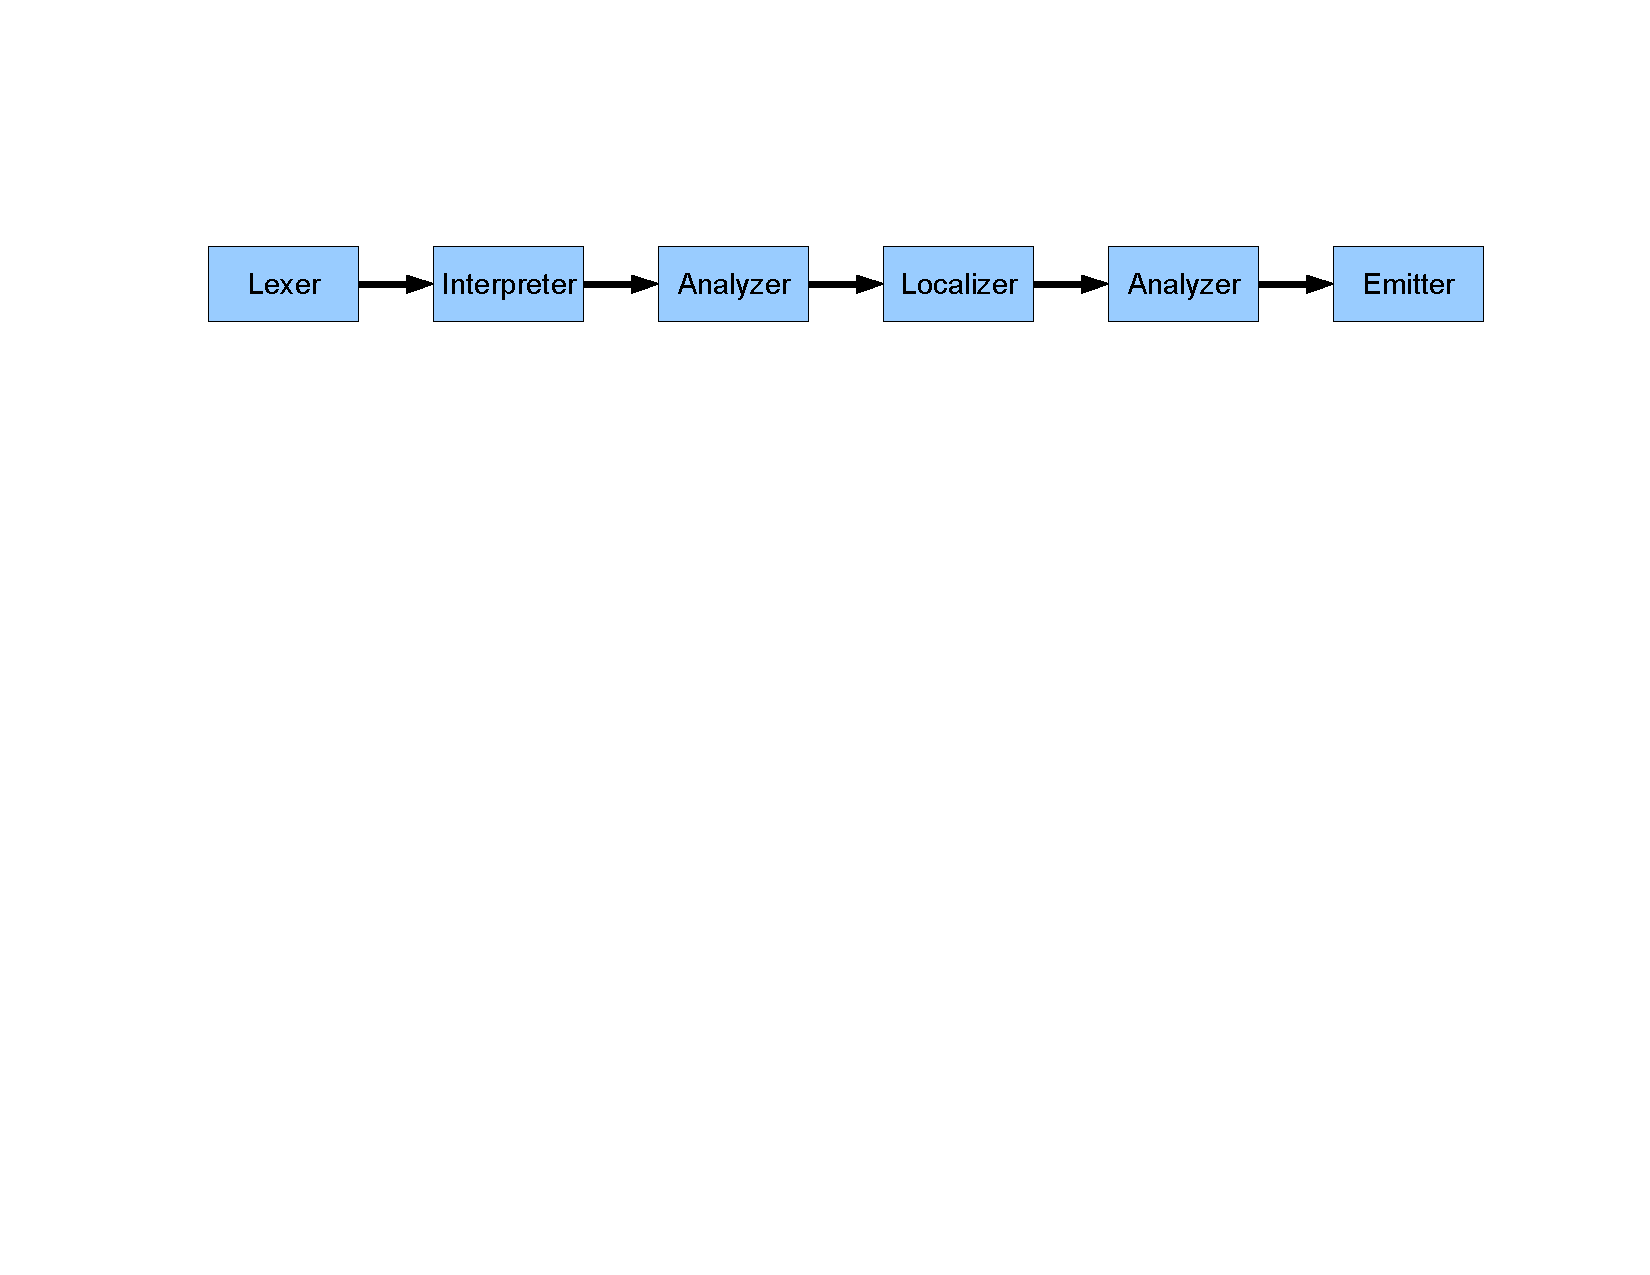
\includegraphics[width=5in]{figures/compiler-phases.pdf}
\caption{The six stages of Proto compilation: the lexer turns text into
tokenized expressions, which is interpreted as a dataflow graph (DFG).  The
analyzer performs type inference and optimization on the DFG, which then
undergoes global-to-local transformation before being run through the analyzer
again.  The resulting localized DFG is then sent to the emitter for
transformation into a platform-specific executable.}
\label{f:compiler-stages}
\end{figure}

\section{Compilation Overview}

The MIT Proto compiler has six stages of compilation, two of which are
duplicates.  These stages, shown in Figure~\ref{f:compiler-stages}, follow a
fairly standard flow of compilation:
\begin{itemize}
  \item The {\bf lexer} turns text into tokenized expressions
  \item The {\bf interpreter} turns expressions into a direct representation of
  the computation.  In the case of Proto, this is a dataflow graph (DFG) of
  operations on fields.
  \item The {\bf analyzer} operates on dataflow graphs, filling in implicit
  information and optimizing.
  \item The {\bf localizer} is a special Proto-specific stage, in
  which the dataflow graph operators are transformed from operations over
  regions of space-time into equivalent operations for a single step on
  individual devices.  The analyzer is run again after the localizer completes.
  \item The {\bf emitter} transforms a localized dataflow graph into a
  platform-specific executable for whatever architecture is being targetted by
  the compiler.  The default architecture is the ProtoKernel VM.
\end{itemize}

\subsection{Compiler Extensions}

The compiler uses DFGs as its central representation, offering the possibility
of alternative emitters or interpreters.  At present, alternate emitters are
supported, but the only emitter bundled in the MIT Proto distribution is the
default emitter, for the ProtoKernel VM.  The BBN BioCompiler, however, is a
Proto emitter that transforms Proto programs into genetic regulatory networks to
implement the program in living biological cells.

The ProtoKernel emitter can also support extensions with device-specific
opcodes, allowing a device's sensors, actuators, and operating system resources
to interact with Proto programs.  At present, however, this is not yet
integrated properly with the simulator's plugin system.

At present, the potential for alternate lexers and/or interpreters has not been
explored.  It is desired, however, as there are many parentheses-phobic
programmers who many be put off by the LISP-like syntax of Proto.  A ``python
skin'' option would likely increase the marketability of Proto without affecting
its semantics in the least.

\subsection{Error Handling}

Like many other compilers, the MIT Proto compiler's error-reporting goal is to
maximize the useful debugging information returned to the programmer at each
compilation.  As such, when errors are discovered, the compiler should report
them but then try to continue work to discover other unrelated errors.
Accordingly, the compiler only checks whether an error has occured after each
stage (or major stage-internal batch of work), and exits gracefully if so.

The {\tt compile\_error} function in \file{compiler-utils.h} should be used to
facilitate this: it reports the error and sets a flag indicating that an error
has occured, ensuring later termination.  When supplied with a {\tt
CompilationElement} (see Section~\ref{s:ce}), it also reports the location of
the error-causing elements in the source code.  Wrapper functions (e.g. {\tt
field\_err}, {\tt type\_err} in \file{ir.h}) are used to also return a dummy
value, allowing compilation to safely proceed to the next checkpoint.

Internal errors, caused by bugs in the compiler, at allowed to terminate
immediately to avoid crashes or corruption.  In order to aid debugging, these
should use the {\tt ierror} function (in \file{compiler-utils.h}) and give a
message that allows the point of failure to be uniquely identified.

\subsection{The {\tt CompilationElement} class}
\label{s:ce}

Error handling and other shared facilities throughout the compiler are enabled
by using the class {\tt CompilationElement} (in \file{compiler-utils.h}) as a
base class for all representions in the compiler.  The {\tt CompilationElement}
class (macro {\tt CE}) provides two basic capabilities: stable ordering
and annotation.

Stable ordering is required for regression testing and consistent cross-platform
operation.  Upon creation, each {\tt CE} is assigned a predictable unique
identifier that can be used to break symmetry in ordering.  Whenever working with a
data-structure that can produce arbitrary orderings, such as an STL {\tt set} or
{\tt map}, the {\tt CompilationElement\_cmp} comparator should be used to order
the elements.  The {\tt CEset} and {\tt CEmap} macros simplify this; see
\file{ir.h} for many examples of their use.

Annotation is a facility for marking representations with additional
informational {\tt Attribute} objects.  Each {\tt CE} stores this information
with a map of string/{\tt Attribute} pairs, and these can be inherited by other
{\tt CE} objects according to rules in each attribute. For example, the lexer
annotates each token with a {\tt Context} attribute containing the source file
and line number that it came from, so that errors and warnings can inform the
programmer what code caused them.  When the interpreter transforms an expression
into a DFG, the DFG elements inherit their {\tt Context} attributes, which union
such that a function knows all of the lines it was written on, not just one.


\section{Lexer}
\label{s:lexer}

The first stage of the compiler is the Lexer, which takes a stream of text and
tokenizes it into formal expressions, discarding comments and whitespace.
Expressions come in three types: symbols, scalars (real numbers, implemented
using floating point), and lists that can contain any mixture of symbols and
scalars.  All expressions are also marked with a ``CONTEXT'' attribute
containing their file/line source location.

Classes representing these expressions are defined in the file \file{sexpr.h},
rooted in {\tt SExpr} (from the LISP ``s-expression'').  Also useful to note is
the {\tt SE\_List\_iter} class, which is designed to simplify later
interpretation of {\tt SExpr} structures.

The lexer is implemented indirectly, using the flex++ lexical parser generator,
in the file \file{proto\_syntax.flex}, which generates \file{lexer.cpp}.  Do not
edit \file{lexer.cpp} directly: your changes will be destroyed the next time
that the file is re-generated.

The lexer groups characters into five batches:
\begin{itemize}
  \item Constituent: alphanumeric and: {\tt * + - .~/ $<$ = $>$ ?~\_ \& :  }
  \item Special: {\tt ; ' ( ) , ` @ $|$}
  \item Reserved: {\tt \textasciitilde~!~" \# \$ \% [ \textbackslash~]
  \{~\textasciicircum~\} }
  \item Whitespace: space, tab, newline variants
  \item All others: unhandled characters producing an error.
\end{itemize}

Whitespace breaks between tokens and is discarded.  A {\tt ;} character
begins a comment: it and everything after until the end of a line are
discarded.  The rest of the characters transform into tokens as follows:
\begin{itemize}
  \item A sequences of constituents produces a scalar or symbol token.  If the
  sequence is an integer, floating point, or scientific ``e'' notation number,
  then it is a scalar.  The tokens {\tt inf}, {\tt Inf}, {\tt -Inf}, {\tt -inf},
  {\tt NaN}, and {\tt nan} also become scalars, with the special IEEE
  floating point values of infinity, negative infinity, and not-a-number
  respectively.  All other sequences become symbols, preserving case for
  alphabetic characters.
  \item The {\tt $|$} character is its own symbol.
  \item Parentheses designate the beginning and end of a list.
  \item The tokens {\tt `}, {\tt '}, {\tt ,}, and {\tt ,@} wrap the next
  expression to make it the second element of a two element list.  The first
  element is a symbol designated by the token: {\tt quasiquote}, {\tt quote}, 
  {\tt comma}, or {\tt comma-splice}, respectively.
  \item Reserved characters produce errors.  At present, \textasciitilde~is
  used internally by the compiler.  The others are unused, but may become
  special characters or be used internally by the compiler at a later date.
\end{itemize}

When there are multiple expressions in a stream, the lexer wraps them together
into a list with initial token {\tt all}, which is the Proto macro for multiple
expression evaluation.

\section{Interpreter}
- DFG model:
 - proto types
  - lattice structure
  - type concreteness [and other properties?]
 - operators, signatures
 - operatorinstances / fields / AMs [+ their macros]
- loading primitives
- reserved symbols
- holding onto needed symbols
- lexical operators
- macro handling

Neighborhood operations (mostly) don't need any special handling.

\paragraph{Restriction Operations}

\begin{figure}
\centering
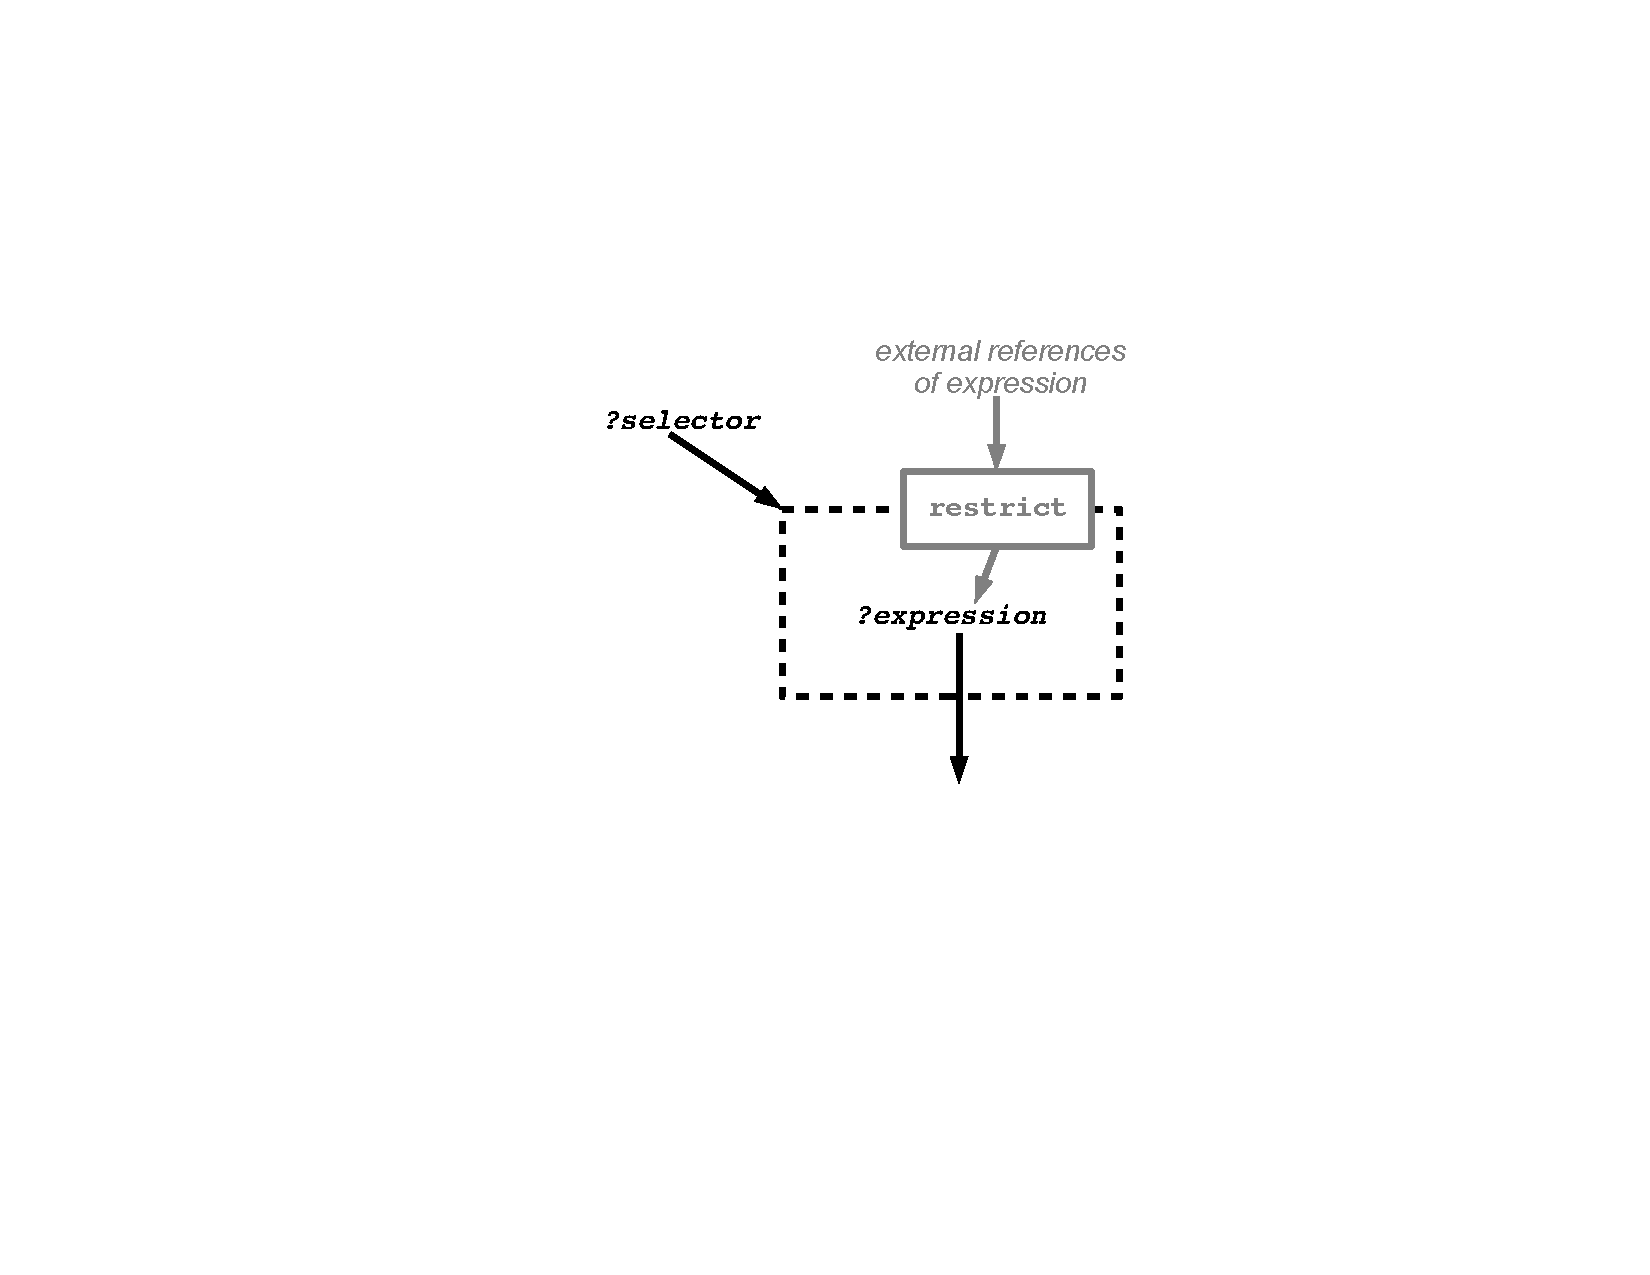
\includegraphics{figures/restriction.pdf}
\caption{}
\label{f:restrict}
\end{figure}

The {\tt restrict} evaluates its expression in a subdomain, as per
Figure~\ref{f:restrict}.

\subsection{Neighborhood Operations} 

\subsection{Feedback Operations}

Feedback operations have a problem: when there is a nbr operation inside
of the update, the nbr exports not the value computed from the current state,
but the value computed from the delayed state during the update.

This is currently made less observable by a paleocompiler/kernel bug: the
paleocompiler generates VM code that runs the update function every time ---
even the first time when only the init code should be running.  As a result, 
the first export happens without delay, though all subsequent ones are delayed.

We will not fix this double-bug until the paleocompiler is deprecated, so that
bug-for-bug compatibility can be preserved across the transition.

When we do fix it, however, the change will actually be to the global semantics,
because that's the portion that's broken.  The most likely fix is to take the
nbr portion of the computation and do it before the delay, so that it gets
exported in the same round.  For many statements, this can be done in a simple
way by the following procedure:
\begin{enumerate}
\item Create two copies of the update expression, one taking delayed
feedback values, one taking non-delayed feedback values.
\item Connect the non-delayed update expression to the feedback mux.
\item Switch the consumers of each nbr in the delayed to its equivalent in the
non-delayed.
\item Allow dead-code elimination to simplify the two branches.
\end{enumerate}
The only problem with this is if there are nbr statements wrapped inside of
compound ops.  Likewise, it is not entirely clear how it should interact
with dt or with nested letfeds.  Thus, this needs more careful thought before we
decide exactly how to proceed.

\section{Analyzer}
- Propagators
- Two passes: pre and post localizer
- Type inference
  - constraints
  - type coercion
- Optimizations

\section{Localizer}

The localizer carries out a key Proto-specific action: it transforms programs
that act over regions of space across periods of time into equivalent programs
that act at a particular point of space at a particular point in time.  

Proto has four space-time families of operations:
\begin{itemize}
  \item Pointwise operations, like {\tt +} and {\tt sqrt}, which involve neither
  space nor time, and therefore transform trivially.
  \item Restriction operations, which reduce the region where a computation is
  executed.  These transform simply into branches, but interact with feedback
  and neighborhood operations.
  \item Feedback operations, which evolve state over time.  These transform into
  storage and recall of state.
  \item Neighborhood operations, which compute over nearby state.  The
  computation over neighbors transforms into a per-neighbor operation, but the
  summary operation remains untouched until the emission stage.
\end{itemize}

\section{ProtoKernel Emitter}
- specifying opcodes
- linearization walk
- propagators
- position resolution

\end{document}
